% article example for classicthesis.sty
\documentclass[10pt,a4paper]{article} % KOMA-Script article scrartcl
\usepackage{lipsum}
\usepackage{url}
\usepackage[nochapters]{classicthesis} % nochapters
\usepackage{graphicx}
\usepackage{float}
\usepackage{subfig}




\begin{document}
    \pagestyle{plain}
    \title{\rmfamily\normalfont\spacedallcaps{Mission: Chuckhole | Personal report}}
    \author{\spacedlowsmallcaps{Marwan El Mezni}}
    \date{} % no date
    
    \maketitle
    
%    \begin{abstract}
        %Maybe we won't need an abstract
 %   \end{abstract}
       
    \tableofcontents


	

    
    \section{Introduction}
	My mission was to overlay the heatmaps and markers in clusters on a google map based on the data structure implemented by Michael.

    \section{Main Reponsibilities}
	
	\subsection{Adding a google map to the app}\label{subsec:map}
	
	To add a google map to an Android app, i followed the following steps :
	\begin{itemize}
		\item Install the Google Play services SDK :
		
		The Google Maps Android API is distributed as part of the Google Play services SDK.
		The Google Maps Android API allowed me to add a Google map into our application. The API automatically handles access to Google Maps servers, data downloading, map display, and response to map gestures. I also utilized API calls to add markers and heatmap overlays on it which will be further detailed in the next sections.
		
		\item Get a Google Maps API key :
		
		To use the Google Maps Android API, I registered our project on the Google API Console and got a Google API key which was added to our app.
		\item Add required settings to the app's manifest "AndroidManifest.xml", I specified:
		
		\begin{itemize}
		\item The Google Play services version that the app will be compiled with.
		\item API key.
		\item Location permissions : 
		
		Our app needs to access the user's location. Android offers two location permissions: "ACCESS COARSE LOCATION" that uses WiFi or mobile cell data (or both) to determine the device's location and "ACCESS FINE LOCATION" which determines a location as precise as possible from the available location providers, including the Global Positioning System (GPS) as well as WiFi and mobile cell data. So, I opted for GPS to get much higher accuracy. 
		
		\end{itemize}
		
        \item Permissions or requirements automatically merged into the manifest at build time : 
        \begin{itemize} 
        \item "INTERNET" : used by the API to download map tiles from Google Maps servers.
        
        \item "ACCESS NETWORK STATE" - allows the API to check the connection status in order to determine whether data can be downloaded.
        
        \item The Google Maps Android API uses OpenGL ES version 2 to render the map.
        
        
        
        
		\end{itemize}
		
		
		
		
		
	
    \item UI controls :
    
	I added UI controls such as : Zoom controls, Compass and the current location of the user button to the map to provide more controls and interaction options. They can be integrated through XML attributes or programmatically. I chose the second alternative.
	
	\item Best known user location :
	
	While displaying the map, the app will try to determine the last known location of the user. First, request permission to access "ACCESS COARSE LOCATION" and "ACCESS FINE LOCATION" described in the previous subsection. Then, in case the GPS is not on, the user will be redirected to the corresponding setting on the phone to activate it. I fixed the choice of a good location provider based on fine accuracy of GPS locations and low power consumption to limit quick discharge of the phone battery.
	
	In case the best known location can't be determined, the app will orientate the map's camera to the center of Passau city.
	
	
	\end{itemize}
	
	\subsection{Heatmap Overlay}\label{subsec:heatmap}

	
	To add a dynamic heatmap to our map, i needed to pass the dataset consisting of the coordinates for each location of interest. This dataset's content vary based on the current zoom level of the map's camera. Using the 'On Camera Change Listener', i fed this method with the current zoom value that will determine if the dataset will be filtered withing a specific zoom range or not before giving its locations as inputs for the overlay.
	\noindent
	Then, i retrieved all locations from the AccFix records of the resulting dataset which will represent the collection of LatLng objects for the HeatmapTileProvider. For the intensity parameter of each object, i divided its corresponding g-force value by 6 to map the intensity range to ]0,1].
	\noindent
	Finally, i just needed to create a new TileOverlay, passing it the heatmap tile provider, and add the tile overlay to the map.
	\noindent
	The radius level was set to its minimum value to reduce even slightly the problem of heatmap overlaps.

	\begin{figure}[H]
    \centering
	   
       	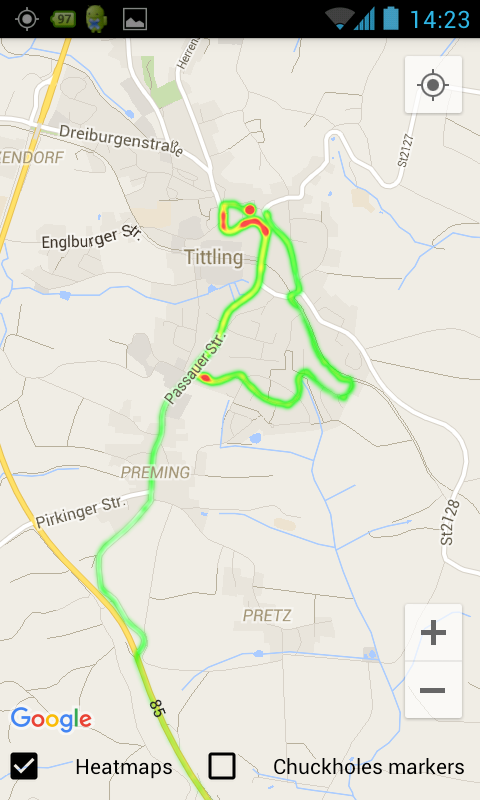
\includegraphics[scale = 0.28]{img/pic4}
       	\caption{Heatmap overlay example}
	\label{fig:heatmap_overlay}
       
    \end{figure}

\subsection{Markers on chuckholes in clusters}\label{subsec:markers}

The marker clustering utility allowed me to manage multiple markers at different zoom levels which will offer a pleasant output and better map readability for the user especially when the number of chuckholes is big.

\noindent
To use the marker clustering utility, I added the java class "ClusterItem" to  represent a marker on the map : returns the position of the marker as a LatLng object. Then, I used a ClusterManager to group the cluster items (markers) based on zoom level. Next, I set the map's OnCameraChangeListener() to the ClusterManager, since ClusterManager implements the listener. Finally, I fed the markers into the ClusterManager, of course only those ones whose corresponding g-force values reach or exceed our threshold = 3.5.

    
    \begin{figure}[H]
    \centering
	
	   
       	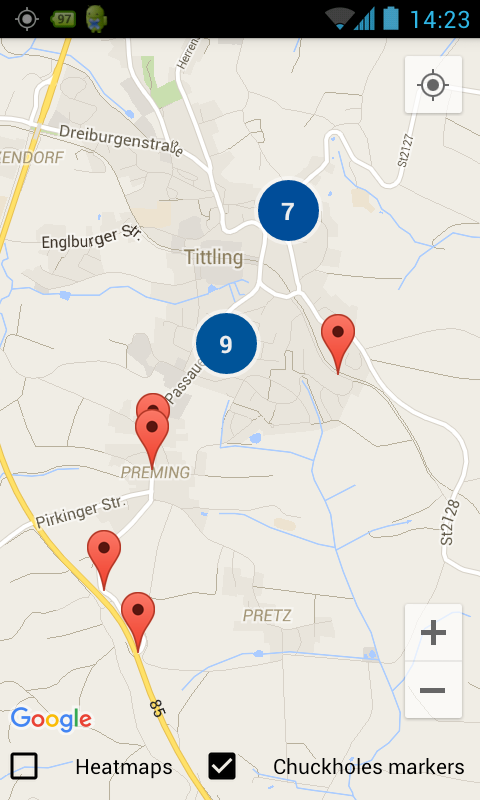
\includegraphics[scale=0.28]{img/pic3}
   	\caption{Markers on chuckholes in clusters}
	\label{fig:markers_overlay1}
	\end{figure}
    
If the recording dataset doesn't contain any chuckholes, the user will get a feedback via a toast message : 

\begin{figure}[H]
    \centering
	
	   
       	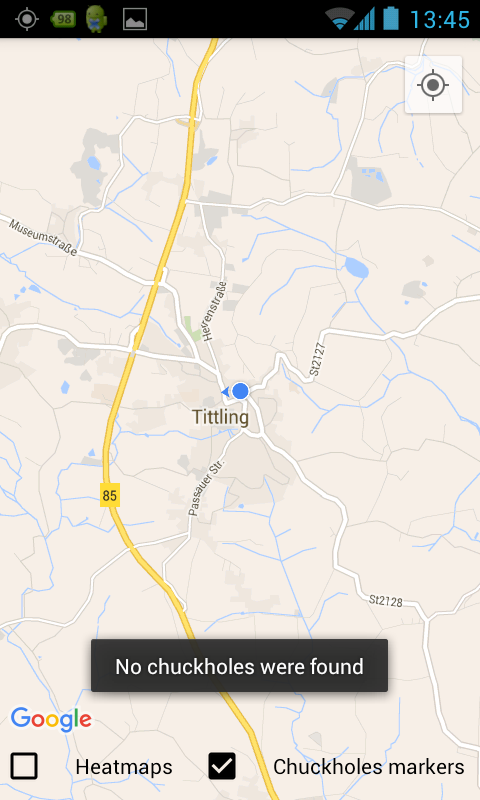
\includegraphics[scale=0.28]{img/pic5}
   	\caption{No chuckholes to overlay}
	\label{fig:markers_overlay2}
	\end{figure}


\subsection{Common report}\label{subsec:report}

The common report was at my charge. Michael helped me by reviewing, commenting and rewording some sections.
    
    \section{Other contributions}

     I contributed to the evaluation of the recording feature by experimenting it along a bike ride around the village where i live.



	
	\section{Problems/Lessons Learned}\label{sec:prob_less}
     \subsection{Problems}\label{subsec:prob}
     
    I had no prior knowledge about mobile development and the last time i developed an app in Java was some years ago. I expected working on this project to be more challenging and exhausting for me compared to some fellow students but i was determined to learn something new and acquire new skills.
    
	\noindent
	The major problem i faced during the implementation phase was with filtering the dataset to overcome the overlapping of heatmaps. I tried a basic solution on my dataset that was created after i tested the recording feature provided by Michael. Unfortunately, it was so dependent on the specific circuit i ride on and thus couldn't be generalized and implemented in the app.
    
    \subsection{Lessons learned}\label{subsec:less}
	This project was a great occasion to get a good overview about mobile development for Android. 
	Now, i'm familiar with Android studio environment and Java programming and got the chance to check the Google Maps API for Android out.





    
    % bib stuff
%    \nocite{*}
%    \addtocontents{toc}{\protect\vspace{\beforebibskip}}
%    \addcontentsline{toc}{section}{\refname}    
%    \bibliographystyle{plain}
%    \bibliography{../Bibliography}
\end{document}
